% GUIDA VELOCE:
% --------------------------------------------------------------------
% X INIZIA UN UNOVO CAPITOLO:
% \chapter{??? NOME CAPITOLO}}
% \section{ ?? }
% \subsection{ ?? }
%
% --------------------------------------------------------------------
% PAROLA CONTENUTA NEL GLOSSARIO:
% scrivere la parola seguita da $^g$
% esempio: User$^g$
%
% --------------------------------------------------------------------
% PER ANDARE A CAPO SENZA RIENTRO INSERIRE:
% \\
%
% --------------------------------------------------------------------
% GRASSETO:
% \textbf{parola}
%
% --------------------------------------------------------------------
% CORSIVO:
% \emph{parola}
% --------------------------------------------------------------------
% PER SCRIVERE IN ROSSO:
% \red{parola}
%
% --------------------------------------------------------------------
% PER SCRIVERE TRA VIRGOLETTE
% ''parola''
%
% --------------------------------------------------------------------
% PER EVITARE IL RIENTRO AUTOMATICO DI UN CAPOVERSO:
% \noindent testo....
%
% --------------------------------------------------------------------

% PER SCRIVERE CARATTERI PARTICOLARI COME: { } _ ecc.. SCRIVERLI PRECEDUTI DA \
% ES: \{ \_
%
% --------------------------------------------------------------------
% X INSERIRE UN LINK:
% \url{http://www.math.unipd.it/~tullio/IS-1/2011/Progetto/C3.pdf}
%
% --------------------------------------------------------------------
% PER COMMENTARE INTERE PARTI:
% \comment{ comment }
%
% --------------------------------------------------------------------
% PER SCRIVERE NOTE DURANTE IL TESTO:
% parola \footnote{ note riguardanti la parola }
%
% --------------------------------------------------------------------
% PER SCRIVERE CODICE SORGENTE:
%
% \lstset{language=c++,
% stringstyle=\color{blue}\textrm,
% commentstyle=\rmfamily, numbers= none}

% \begin{lstlisting}
% CODICE
% \end{lstlisting}
%
% --------------------------------------------------------------------
% !!!!!!!! PER COSE + COMPLESSE VEDI: !!!!!!!!!!!!!!!!!!!!!!!
% !!!!!!!! PMAC/latex/GUIDA LATEX!!!.tex !!!!!!!!!!!!!!!!!!!!!!!

% per tutto il resto chiedi a lory prima di fare/scrivere cazzate !!!!!!!!!!



\documentclass[10pt,a4paper]{article}

\usepackage[italian]{babel}
\usepackage[T1]{fontenc}
\usepackage[utf8x]{inputenc} % uso utf8x xk x linux, mentre latin1 è per windows
\usepackage{lmodern} %insieme di font molto completo consigliato da LatexFacile pg13 in basso
\usepackage{microtype} %migliora riempimento delle righe. vedi LatexImpaziente pg41
%attiva il rientro di ogni prima riga di ogni sezione: capitolo,paragrafo ecc. vd LatexImpaziente pg41
\usepackage{indentfirst}
\usepackage{graphicx} % per inseire immagini
\usepackage[usenames,dvipsnames]{color}
\usepackage{lastpage} %serve per poter scrivere page 1 of N
% setta i bordi della pagina: dx e sx 3.2cm di rientro + nel lato di rilagatura rientra di altri 0mm
\usepackage[a4paper,top=3cm,bottom=3cm,left=3.2cm,right=3.2cm, bindingoffset=0mm]{geometry}
\usepackage{listings} % per inserire codice sorgente
\usepackage{float} % per gestire oggetti flottanti ( es immagini tabelle posizionebili con "H" che forza il posizionamento nel punto specifico )

% serve per creare tabelle lunghe + di una pagina con \begin{longtable} (vd Tabelle.pdf pg11-12)
\usepackage{longtable}

\usepackage{fancyhdr} % per impostare lo stile della pagina più personalizzato, + fancyhdr ( per regolare testatina e piè di pagina ) vedi itfancyhrd



\pagestyle{fancy}
% settaggi di pagestyle(fancy)
\lhead{
\includegraphics[scale=0.20]{images/SevenFold_small}}
%\chead{}
\rhead{\textbf{{%
\NomeDocumento - \VersioneAttuale \\ Data versione attuale: \DataRilascio \\ e-mail: \mail{sevenfold@palomino.it}}}}
\lfoot{\NomeDocumento}
\cfoot{}
\rfoot{ \textbf \thepage\ di \pageref{LastPage}}
\renewcommand{\footrulewidth}{0.4pt}

%ridefinisco il plain per cosare l'indice (a questo punto si potrebbe lasciare tutto il documento in plain
\fancypagestyle{plain}{
\lhead{
\includegraphics[scale=0.20]{images/SevenFold_small}}
%\chead{}
\rhead{\textbf{{%
\NomeDocumento - \VersioneAttuale \\ Data versione attuale: \DataRilascio \\ e-mail: \mail{sevenfold@palomino.it}}}}
\lfoot{\NomeDocumento}
\cfoot{}
\rfoot{ \textbf \thepage\ di \pageref{LastPage}}
\renewcommand{\footrulewidth}{0.4pt}
}

% da ultimo:
\usepackage{hyperref} %x l'interpretazione di indirizzi o link ipertestuali (vd LatexImpaziente pg47 )
\hypersetup{backref, colorlinks=true, linkcolor=black, urlcolor=black}

\usepackage{url} % x l'interpretazioni di internet o link ipertestuali (vd LatexImpaziente pg47 )
%\UrlFont{color =blue}
%\urlstyle{helvetic}

% Define a new 'leo' style for the package that will use a smaller font.
\makeatletter
\def\url@leostyle{%
  \@ifundefined{selectfont}{\def\UrlFont{\sf}}{\def\UrlFont{\small\ttfamily}}}
\makeatother
%% Now actually use the newly defined style.
\urlstyle{leo}


\newcommand{\mail}[1]{\textcolor{Black}{ \texttt{#1}}} %per interpretare mail (vd LatexImpaziente pg47 )
\newcommand{\cambiaFont}[2]{{\fontencoding{T1}\fontfamily{#1}\selectfont#2}}
\newcommand{\red}[1]{ \textcolor{red}{#1} } % per scrivere testo in rosso
\newcommand{\comment}[1]{} % per inserire commenti

\newcommand{\attribute}[2]{ \item[\textcolor{PineGreen}{ \texttt{#1}}] \textcolor{PineGreen}{\texttt{#2\\}}\ \ \ }
\newcommand{\method}[2]{ \item[\textcolor{MidnightBlue}{ \texttt{#1}}] \textcolor{MidnightBlue}{ \texttt{#2\\}}\ \ \ }

\newcommand{ \class}[1]{ \item[-] \texttt{#1} }
\newcommand{\virgolette}[1]{``{#1}''}



% INSERIRE QUI IL NOME DEL DOCUMENTO SEGUITO DA UNO SPAZIO
% ( così il nome si imposta in automatico nelle varie ricorrenze standard)
\newcommand{\NomeDocumento}{Scrivi in questo documento k poi uniamo tutto }

% INSERIRE QUI LA DATA DEL RILASCIO DELLA VERSIONE ATTUALE
\newcommand{\DataRilascio}{2012/04/02}

% INSERIRE LA VERSIONE ATTUALE
\newcommand{\VersioneAttuale}{v2.0.0}

% INSERIRE QUI L'ACRONIMO DEL DOCUMENTO. ESEMPIO: Analisi Dei Requisiti = AR
% Quando inserite l'acronimo qui, dovete rinominare i file presenti nella cartella
% del tipo '??-cap1-NomeCapitolo.tex' sostituendo i '??' con l'acronimo scelto!!
\newcommand{\AcronimoDocumento}{DP}

\begin{document}


% --------------------------------------------------------------------

% TITOLO ( 1° pagina)

\vspace*{2.5cm}
\begin{center}

%\cambiaFont{Cyklop}{Sevenfold}
%\cambiaFont{fve}{\Huge{Sevenfold}}

\includegraphics[scale=0.35]{images/SevenFold_big}

\vspace{2cm}

\cambiaFont{fve}{\Huge{\NomeDocumento}}\\
\vspace*{1cm}

è richiesto: circa 15 pagine a testa..

\end{center}


% --------------------------------------------------------------------

% INFORMAZIONI DEL DOCUMENTO ( 1° pagina)

\vspace*{2cm}




% --------------------------------------------------------------------

% SOMMARIO ( 2° pagina)

\newpage

\vspace*{0.5cm} % il vertical space va preceduto da una riga vuota!!!
\begin{center}

\textbf{{\huge{Sommario}}}
------------------------EMPTY-------------------------

\vspace*{0.2cm} % il vertical space va preceduto da una riga vuota!!!

\end{center}


% --------------------------------------------------------------------



% --------------------------------------------------------------------
% INDICI:

\newpage

% INDICE CAPITOLI
\tableofcontents % genera l'indice di tutto il documento

\let\cleardoublepage\clearpage % toglie la pagina bianca dopo l'indice

% INDICE TABELLE
\listoftables

% INDICE FIGURE
\listoffigures


% --------------------------------------------------------------------

% LORY LA MIA PARTE INIZIA DA QUA E PRIMA DI QUA CI DEVI METTERE IL SOMMARIO E LE ALTRE STRONZATE

\newpage
\section{Introduzione}


\subsection{Scopo del documento}
Il presente documento rappresenta un Business Plan per il sistema denominato \textbf{Woty},  sviluppato dal teamwork Sevenfold in corrispondenza del corso di Ingegneria del Software [2012].\\





\section{Descrizione del Sistema}

Descriveremo ora le funzionalità pratiche del sistema, dagli attori coinvolti ai vari ambiti di utilizzo, al fine di rendere chiaro a un soggetto esterno l'effettiva utilità del prodotto.

\subsection{Cos'è Woty}

Il sistema software Woty si pone come obiettivo la realizzazione di una piattaforma innovativa per l’apprendimento comportamentale nell’ambito della sicurezza del lavoro, che utilizzi le tecniche della gamification per incentivare il coinvolgimento e la partecipazione degli utenti e per scardinare l’instaurarsi di abitudini errate.\\
Woty è orientato alla ”quest ”, che consiste in un compito/sfida che l’utente dovrà compiere.\\
Questo permetterà al sistema di assegnare un punteggio, che concorrerà alla creazione di classifiche personali o di gruppo.\\
Woty vuole poter essere utilizzato sia in ambito aziendale su postazioni fisse (indipendentemente dall’OS utilizzato), sia in ambito mobile, attraverso l’utilizzo di smartphone.\\

\subsection{Collocazione del prodotto}

Il sistema software Woty può essere adottato da qualsiasi realtà lavorativa dove l’uso del computer rientra nella normale routine dei dipendenti. \\
I clienti che decidono di usare Woty offrono ai loro impiegati la possibilità di sostituire un eventuale corso frontale sulla sicurezza con l’utilizzo del nostro sistema.\\
In ambito aziendale la formazione del personale riguardo conoscenze critiche, come può essere ad esempio la gestione delle norme sulla sicurezza sul lavoro, è normalmente erogata secondo procedure statiche scollegate dall’ambiente lavorativo come l’insegnamento in aula, che poco motivano e stimolano all’apprendimento i partecipanti.\\
Un apprendimento diverso, di forma continua e interattiva, può essere erogato ai lavoratori come parte integrante delle attività lavorative standard, per fare in modo che il coinvolgimento dell’utente sia elevato, grazie a compiti e sfide a cui verrà sottoposto.\\
Un aumento dell’interesse e della partecipazione del lavoratore può essere creato attraverso elementi di gamification ,con i quali verrà innestata una forma di competizione tra le diverse squadre di lavoro, oltre che nel singolo.

\subsection{Funzionalità del prodotto}

Di seguito sono descritte in generale le funzionalità che il sistema fornisce ai suoi utenti.\\

\subsubsection{Ambiente aziendale}
Nell’ambiente aziendale, Woty permette agli User di portare a termine le quest direttamente all’interno di un browser. Un sistema di notifica nel terminale dello User lo informa della presenza di nuove quest disponibili. Il sistema di notifica gestirà anche l’autenticazione al sistema.\\ 
È prevista in ogni azienda la presenza di un Super-userg per l’amministrazione delle utenze.\\


\subsubsection{Ambiente mobile}
Gli User in mobilità denominati Mobile-user , tramite l’applicazione dedicata, si autenticano, svolgono le quest loro assegnate e visualizzano statistiche e punteggi esattamente come farebbero con la normale interfaccia desktop.

\subsection{Ambiente di esecuzione}

Il software è sviluppato sul modello client-server. I client si dividono in desktop e mobile. La parte server è ospitata unicamente presso le macchine del fornitore.\\
L’inserimento di un nuovo cliente comporta un intervento sull’interfaccia web da parte del Woty Administrator, che fissa inoltre il numero di account istanziabili dal nuovo cliente.\\
Viene designato un Super-user presso il cliente che tramite un’interfaccia web avrà le responsabilità di:
\begin{itemize}
\item{ Assegnare i singoli account utente al personale. }
\item{ Associare ad ogni account un workgroup che ne identifica il dipartimento (e.g. impiegato, operaio, etc.) scelta da un pool di workgroup assegnato all’azienda dal Woty Administrator. }
\end{itemize}

A questo punto la normale amministrazione del sistema è in mano al Super-user, che non dovrebbe avere bisogno del fornitore a meno di guasti.

\subsubsection{Server}
Il software va installato, inizializzato e testato presso i server scelti dal 	fornitore del servizio.\\
L’uso è ridotto alla gestione amministrativa tramite interfaccia web, che deve poter essere portata a termine anche da personale qualificato ma non necessariamente tecnico.\\

\newpage

\subsection{Client Desktop}
Dopo l’assegnazione di un account da parte del Super-user, il primo contatto dello User con il sistema è la visita alla homepage del software che aiuta, tramite un wizard , l’installazione del demone per la gestione dell’autenticazione e delle notifiche.\\
Come riportiamo nei dati a seguire, vista la larga diffusione e uso della rete internet nel nostro paese, si presuppone che un utente medio sia in grado di svolgere senza difficoltà tutte le operazioni richieste, quindi non dovrebbe essere necessario l’aiuto di personale specifico per i passi precedentemente descritti.\\
Da questo punto per l’utente può cominciare la partecipazione attiva.\\


\begin{figure}[H]
\centering
\caption{Statistiche ufficiali Api}
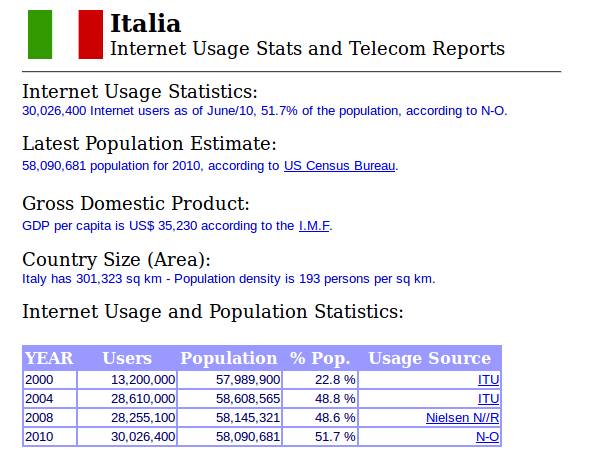
\includegraphics[scale=0.55]{images/statItaly} 
\end{figure}

Inoltre, l'interfaccia web sarà sviluppata tale da rimanere inalterata se visualizzata con diversi browser, anche con differenti versioni.\\
Riportiamo di seguito le statistiche percentuali sull'utilizzo dei browser aggiornate a giugno 2012.

\begin{figure}[H]
\centering
\caption{Statistiche ufficiali Api}
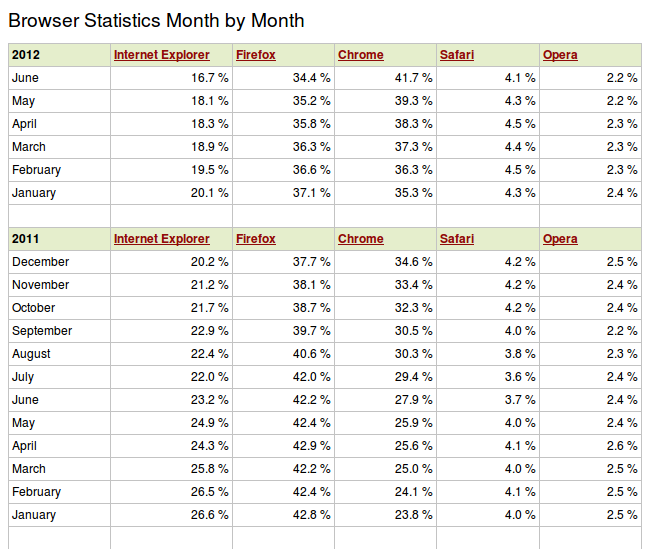
\includegraphics[scale=0.55]{images/internetStat} 
\end{figure}


\subsubsection{Client Mobile}
Per ogni dispositivo è disponibile un client distribuito a seconda della piattaforma in uso.\\
Dopo la canonica inizializzazione e assegnazione di un account da parte del Super-user, lo User può direttamente autenticarsi e cominciare a operare tramite l’interfaccia dell’applicazione.\\ 
Un Mobile-user ha inoltre la facoltà di agire esattamente come un Desktop-user tramite l’interfaccia web.\\
Dopo un'attenta valutazione e in base ai criteri di seguito esposti, abbiamo deciso di sviluppare l'applicazione solo su dispositivi Android, data la limitazione derivante dalle risorse concesse.\\
Nulla vieta, in futuro, di poter sviluppare l'applicazione anche per diversi sistemi.

\begin{figure}[H]
\centering
\caption{Statistiche d'uso dispositivi Android}
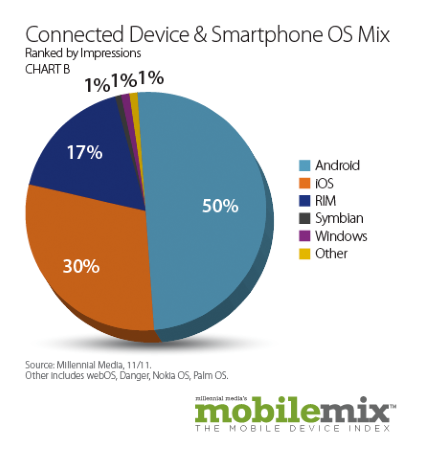
\includegraphics[scale=0.50]{images/statAndroid} 
\end{figure}

Per quanto riguarda la scelta della versione da utilizzare abbiamo seguite le seguenti statistiche; gli aspetti tecnici tuttavia verranno trattati più dettagliatamente nei prossimi capitoli.\\

\begin{figure}[H]
\centering
\caption{Statistiche ufficiali Api}
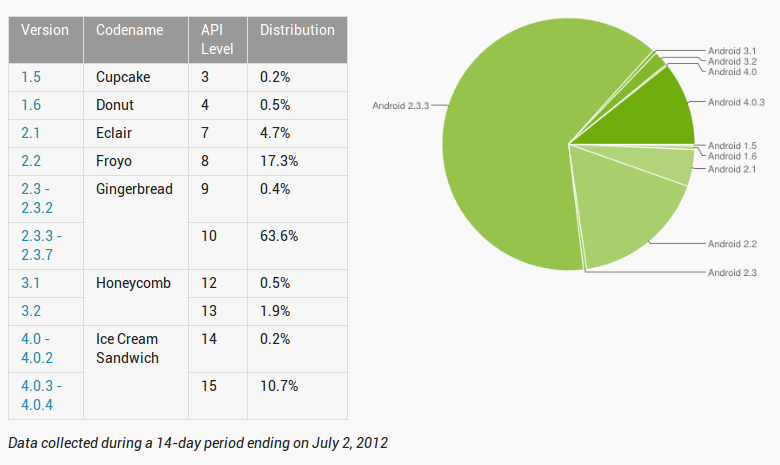
\includegraphics[scale=0.55]{images/api} 
\end{figure}

\newpage

\subsection{Caratteristiche degli utenti}
Gli attori chiamati in causa si suddivideranno nelle seguenti categorie:

\begin{enumerate}

\item Woty Administrator\\
L'attività assegnata al Woty Administrator è quella di illustrare il funzionamento del software presso il cliente ed eventualmente aiutare ad installare le applicazioni mobile.\\
E' incaricato dell'inserimento delle quest. Conoscenze pratiche richieste: gestione di sistemi e reti informatiche.\\

\item Desktop-user, a loro volta divisi in:

\begin{enumerate}

\item Desktop-user senza dispositivo mobile\\
Questo tipo di attore dovrà svolgere le varie quest assegnategli da postazione fissa;

\item Desktop-user con dispositivo mobile\\
Questo tipo di attore dovrà svolgere le varie quest assegnategli, inoltre potrà averne a disposizione altre specifiche in cui si richiede l'uso di un dispositivo mobile (e.g. rilevamento di QR-Code).

\end{enumerate}

\item Mobile-user\\
Questa tipologia di utenti potrà svolgere le proprie quest direttamente dal dispositivo mobile, quindi senza essere fisicamente nell'azienda.

\paragraph{}
Per entrambi gli attori Desktop-user e Mobile-user non sono richieste particolari conoscenze informatiche.

\item Super-user\\
Il Super-user sarà colui che all'interno dell'azienda dovrà occuparsi di visionare i risultati delle varie quest ed eventualmente illustrarne il funzionamento agli User. Si occupa inoltre dell'assegnazione di workgroup agli User del sistema.

\end{enumerate}

\newpage

\subsection{Descrizione quest}

Le tipologie di quest che un User può sostenere sono varie, caratterizzate da un input che Woty darà all'utente e da una risposta che l'utente darà al sistema, in base alle richieste.\\
SevenFold si riserva di ampliare e/o modificare le tipologie di quest offerte durante lo sviluppo di Woty, a seguito di decisioni prese in sinergia con la ditta proponente.\\

\subsubsection{Caratterizzazione in base all'input Woty -> User}
\begin{itemize}
\item Testo: l'User visualizzerà un semplice testo.
\item Foto: l'User visualizzerà a video un'immagine.
\item Video: l'User visualizzerà un filmato.
\end{itemize}

\subsubsection{Caratterizzazione in base alla risposta dell'User}
\begin{itemize}
\item Risposta secca (si/no, vero/falso)
\item Risposta chiusa tra un certo numero alternative
\item Risposta multipla tra un certo numero di opzioni
\item In caso di quest basata su testi, possibilità di riordinare testi disordinati
\item In caso di quest basata su foto, possibilità di riordinare foto spezzettata e disordinata (puzzle)
\item Scansione di un QR-Code$^g$ (Mobile-user)
\end{itemize}

\subsubsection{Caratterizzazione in base al tempo di risoluzione}
\begin{itemize}
\item Standard: quest senza un limite di tempo di risoluzione.
\item Temporizzata: quest con un limite di tempo di risoluzione.
\end{itemize}




\end{document}
